\documentclass{shortart}

\usepackage{amsthm, amsmath, amssymb}
\usepackage[titletoc]{appendix}
\usepackage{tikz-cd}
\usepackage{tikz}
\usepackage{plastex}

\author{Dexter Chua}
\title{The Heat Kernel}

\renewcommand\labelenumi{(\roman{enumi})}
\renewcommand\theenumi\labelenumi

\newtheorem{thm}{Theorem}[section]
\newtheorem{lemma}[thm]{Lemma}
\newtheorem{prop}[thm]{Proposition}
\newtheorem{cor}[thm]{Corollary}
\theoremstyle{definition}
\newtheorem{eg}[thm]{Example}

\newcommand\bra\langle
\newcommand\ket\rangle
\newcommand\loc{\mathrm{loc}}
\newcommand\R{\mathbb{R}}
\newcommand\Z{\mathbb{Z}}
\newcommand\C{\mathbb{C}}
\renewcommand\d{\mathrm{d}}
\renewcommand\Re{\mathrm{Re}}

\DeclareMathOperator\coker{coker}
\DeclareMathOperator\dom{dom}
\DeclareMathOperator\im{im}
\DeclareMathOperator\idx{index}
\DeclareMathOperator\sign{sign}
\DeclareMathOperator\tr{tr}
\DeclareMathOperator\vol{vol}
\DeclareMathOperator\erfc{erfc}

\begin{document}
On a closed Riemannian manifold, there are three closely related objects we can study:
\begin{enumerate}
  \item Topological invariants such as the Euler characteristic and the signature;
  \item Indexes of differential operators; and
  \item Differential forms on the manifold.
\end{enumerate}

(i) and (ii) are mainly related by the Hodge decomposition theorem --- the signature and Euler characteristic count the dimensions of the cohomology groups, and Hodge theory says the cohomology groups are exactly the kernels of the Laplacian. This is explored briefly in Appendix \ref{section:index-and-geometry}.

(i) and (iii) are related to each other via results such as the Gauss--Bonnet theorem and the Hirzebruch signature theorem. The Gauss--Bonnet theorem says the Euler characteristic of a surface is the integral of the curvature; The Hirzebruch signature theorem says the signature is the integral of certain differential forms called the $L$-genus, given as a polynomial function of the Pontryagin forms.

(ii) and (iii) can also be related directly to each other, and this connection is what I would call ``index theory''. The main theorem is the Atiyah--Singer index theorem, and once we have accepted the connection between (i) and (ii), we can regard the Gauss--Bonnet theorem and the Hirzebruch signature theorem as our prototypical examples of index theory.

I wish to make the point that (i) and (ii) are purely global invariants, in the sense that we can only make sense of them when we are given the manifold as a whole. On the contrary, the construction in (iii) is purely local. As long as we construct the Pontryagin form using Chern--Weil theory, the differential forms are globally defined up to equality, and not just up to exact forms.

Thus, it makes sense to ask the following question --- if we are given a compact Riemannian manifold \emph{with boundary}, we can still integrate the differential form we had above. The signature still makes sense, and we can ask how these two relate.

We do not expect them to be equal. In the case of a surface $M$ with boundary, Gauss--Bonnet says
\[
  \chi(M) = \int_M K \;\d x + \int_{\partial M} \sigma \;\d s,
\]
where $K$ is the Gaussian curvature and $\sigma$ is the geodesic curvature of the boundary. However, if the neighbourhood of the boundary is isometric to the product $\partial M \times [0, 1]$, then the boundary term vanishes, and so the Euler characteristic is just the integral of the curvature.

For the signature, even if we assume the boundary is isometric to a product, the integral of the $L$-genus still does not give the signature. However, the difference between the two is entirely a function of the Riemannian manifold $\partial M$. Indeed, if we have two manifolds $M, M'$ with the same boundary, and both are isometric to products near the boundary, then we can glue them together along the boundary. Since both the signature and the integral of the $L$-genus add up when we glue manifolds along boundaries, the error terms of $M$ and $M'$ must be the same.

It turns out this error term is a \emph{spectral} invariant. We can define an elliptic self-adjoint operator $A$ on $\Omega^*(\partial M)$ which, up to some signs, is $\d * + * \d$. We can define
\[
  \eta(s) = \sum_{\lambda \not= 0} \sign \lambda\, |\lambda|^s,
\]
where we sum over the eigenvalues of $A$ with multiplicity. This converges when $\Re (s)$ is large, and has a meromorphic continuation to all of $\C$. We will show that the error term is then $\frac{\eta(0)}{2}$.

Our strategy to understanding this is to employ the heat kernel, which is a way of understanding the connection between (ii) and (iii). In Section \ref{section:heat-equation}, we discuss the classical heat equation and construct the heat kernel on a general closed manifold. From that particular construction, it will be evident how the heat kernel is related to the index of a differential operator. In Section \ref{section:heat-kernel-laplacian}, we provide an alternative construction of the heat kernel of the Laplace--Beltrami operator, which gives us some precise estimates. In Section \ref{section:unbounded-domain}, we use the estimates to construct a heat kernel for the Laplacian on open manifolds. This section is merely an example of what one can do with the estimates, and the results are not used anywhere else. In Section \ref{section:hirzebruch}, we use our results in Section \ref{section:heat-equation} and \ref{section:heat-kernel-laplacian} to prove Hirzebruch's signature theorem.

In Section \ref{section:signature-with-boundary}, we begin to study the signature on a manifold with boundary and connect this to the index of an operator, which we of course hope to calculate using the heat kernel. This is rather more complicated than what one might initially think. In Section \ref{section:on-boundary}, we study the heat kernel on a manifold of the form $N \times \R_{\geq 0}$, which we think of as the collar neighbourhood of a manifold. In Section \ref{section:with-boundary}, we glue the results of the previous chapter with results on the interior established early on to understand the heat kernel on manifolds with boundary, and finally apply this theory to prove the theorem stated above.

To give credit where credit is due, Section \ref{section:heat-kernel-laplacian} is essentially lifted straight out of \cite[Section 4]{patodi-curvature}; Section \ref{section:unbounded-domain} out of \cite{dodziuk-maximum}. The rest of the work is cherry-picked out of \cite{atiyah-bott-patodi} and \cite{atiyah-patodi-singer} (see also \cite{atiyah-bott-patodi-errata} for an errata to \cite{atiyah-bott-patodi}).

\section{The Heat Equation}\label{section:heat-equation}
\subsection{The Classical Heat Equation}
In the most classical sense, the heat equation is the following partial differential equation on $\R^d \times \R$:
\[
  \left(\frac{\partial}{\partial t} - \sum \frac{\partial^2}{\partial x_i^2}\right)f = 0.
\]
This describes the dispersion of heat over time, where $f(x, t)$ is the temperature at position $x$ at time $t$. To simplify notation, we write
\[
  \Delta = - \sum \frac{\partial^2}{\partial x_i^2}.
\]

Green's strategy to solving such a PDE is to find a solution to the PDE with initial condition
\[
  f(x, 0) = \delta (x).
\]
In this case, we can find it very explicitly to be
\[
  f(x, t) = \frac{1}{(4\pi t)^{d/2}} \exp \left(-\frac{|x|^2}{4t}\right).
\]
We call this $H_t(x)$. Then given any bounded continuous function $f_0$, it is easy to see that the solution to the initial value problem
\[
  f(x, 0) = f_0(x)
\]
is simply given by
\[
  f(x, t) = \int_{\R^d} H_t(x - y) f_0(y)\;\d y.
\]

The fact that we are allowed to write $H_t(x - y)$ at all uses the fact that we are working on $\R^d$ and our system has translational symmetry. In general, if we work on an arbitrary manifold $M$, we would seek a function $H_t(x, y)$ on $M \times M \times (0, \infty)$ such that the solution to the initial value problem $f(x, 0) = f_0(x)$ is
\[
  f(x, t) = \int_M H_t(x, y) f_0(y)\;\d y.
\]
The function $H_t(x, y)$ then satisfies
\[
  \left(\frac{\partial}{\partial t} + \Delta_x\right) H_t(x, y) = 0.
\]
This $H_t(x, y)$ is also called the \emph{heat kernel}, or \emph{fundamental solution}, and we will mostly use these terms interchangeably. (It is also called a \emph{Green's function}, but we will not use this name)

The heat kernel also shows up in a closely related problem. Suppose we wanted to solve instead
\[
  \left(\frac{\partial}{\partial t} - \Delta\right)f = F(x, t)
\]
for some (bounded continuous) forcing term $F$. It turns out the solution can also be expressed in terms of $H$ as
\[
  f(x, t) = \int_M H_t(x, y) f_0(y)\;\d y + \int_0^t \d \tau \int_M H_{t - \tau}(x, y) F(y, \tau) \;\d y,
\]
which is again not difficult to check. The interpretation of this is that we can think of the forcing term as adding a new initial condition at each point $\tau$ in time. This is known as \emph{Duhamel's principle}.

Especially from a physical perspective, it is interesting to note that the heat equation propagates information at infinite speed. In other words, for any $t > 0$, the value of $f(x, t)$ depends on the values of $f_0$ \emph{everywhere}. This is in contrast with, for example, the wave equation, where information only propagates at finite speed. Nevertheless, in the limit $t \to 0$, the asymptotic behaviour is purely local, as the contribution of the points a finite distance away decays exponentially as $t \to 0$.

On a general Riemannian manifold, we can formulate the same problem, replacing $\Delta$ by the Laplace--Beltrami operator. The Laplace--Beltrami operator (or Laplacian for short) can in fact be defined for all $p$-forms. Write $\Omega^* = \bigoplus_p \Omega^p$.\footnote{We will abuse notation and write $\Omega^p$ for both $\bigwedge^p T^*M$ and its global sections} Then the exterior derivative defines a map
\[
  \d\colon \Omega^* \to \Omega^*.
\]
There is an $L^2$ inner product on $p$-forms coming from the metric, and so $\d$ has a formal adjoint $\d^*\colon \Omega^* \to \Omega^*$ that lowers degree by $1$. The Laplace--Beltrami operator is given by
\[
  \Delta = (\d + \d^*)^2 = \d^* \d + \d \d^* \colon \Omega^p \to \Omega^p.
\]
In the case of $p = 0$, the Laplace--Beltrami operator is simply given by $\d^* \d$, and in local coordinates with metric $g$, we can write this as
\[
  \Delta f = \frac{1}{\sqrt{\det g}} \partial_i (\sqrt{\det g}\, g^{ij} \partial_j f).
\]

\subsection{The General Heat Equation}
We can further generalize our previous problem and replace $\Delta$ by any elliptic self-adjoint operator. We will soon specialize to the case of the Laplace--Beltrami operator, but this section is completely general.

Our original motivation was to understand the index of operators, so let us start from there. Suppose we are given a compact Riemannian manifold $M$ and $E, F$ Hermitian vector bundles on $M$. We are also given an elliptic differential operator $D\colon \Gamma(E) \to \Gamma(F)$ over $M$ with formal adjoint $D^*\colon \Gamma(F) \to \Gamma(E)$ (in the case of the Laplace--Beltrami operator, we have $D = D^* = \d + \d^*$ and $E = F = \Omega^*$). 

Similar to the case of the Laplace--Beltrami operator, we define
\[
  \begin{aligned}
    \Delta_E &= D^* D \colon \Gamma(E) \to \Gamma(E)\\
    \Delta_F &= D D^*\colon \Gamma(F) \to \Gamma(F).
  \end{aligned}
\]
Then $\ker \Delta_E = \ker D$ and $\ker \Delta_F = \ker D^*$. So we have
\[
  \begin{aligned}
    \idx D &= \dim \ker D - \dim \coker D \\
    &= \dim \ker D - \dim \ker D^*\\
    &= \dim \ker \Delta_E - \dim \ker \Delta_F.
  \end{aligned}
\]
This is the form of the index that will be of interest to us.

By analogy with the classical heat equation, we consider the equation
\[
  \left(\frac{\partial}{\partial t} + \Delta_E\right) f = 0
\]
on $E \times (0, \infty) \to M \times (0, \infty)$, with $t \in (0, \infty)$.

Hodge theory gives us an easy way to solve this, at least formally. We can decompose
\[
  L^2(E) = \bigoplus_\lambda \Gamma_\lambda(E),
\]
where $\Gamma_\lambda(E)$ is the $\lambda$-eigenspace of $\Delta_E$. The spectral theorem tells us the eigenvalues are discrete and tend to infinity. Let $\{\psi_\lambda\}$ be an orthonormal eigenbasis. Then we can write a general solution as
\[
  f(x, t) = \sum_\lambda c_\lambda e^{-\lambda t} \psi_\lambda(x)
\]
for some constants $c_\lambda$.

If we want to solve this with initial condition $f_0$, i.e.\ we require $f(-, t) \to f_0$ as $t \to 0$ in $L^2$, then we must pick\footnote{This requirement is rather weak. We will later upgrade this to a pointwise convergence}
\[
  f(x, t) = \sum_\lambda e^{-\lambda t} \psi_\lambda(x) \bra \psi_\lambda, f_0\ket.
\]
Thus, we can write the heat kernel as
\[
  H_t(x, y; \Delta_E) = \sum_\lambda e^{\lambda t} \psi_\lambda(x) \psi_\lambda(y)^T.
\]
Then we have
\[
  f(x, t) = \int_M H_t(x, y; \Delta_E) f_0(y)\;\d y.
\]
We remark that for each fixed $t$, the heat kernel $H_t(x, y)$ is a section of the exterior product $E \boxtimes E^* \to M \times M$.

To ensure the sum converges, we need to make sure the eigenvalues grow sufficiently quickly. This is effectively Weyl's law, but we for our purposes, we can use a neat trick to obtain a weaker bound easily.
\begin{lemma}\label{lemma:weyl-law}
  If $\Delta$ is any self-adjoint elliptic differential operator, then there is a constant $C$ and an exponent $\varepsilon$ such that for large $\Lambda$, the number of eigenvalues of magnitude $\leq \Lambda$ is at most $C \Lambda^\varepsilon$.
\end{lemma}

\begin{proof}
  To simplify notation, we assume $\Delta$ acts on the trivial line bundle. By replacing $\Delta$ with its powers, we may assume that the order $d$ of $\Delta$ is large enough such that we can apply the Sobolev (and regularity) bound
  \[
    \|f\|_{C^0} \leq C' \|f\|_d \leq C (\|\Delta f\|_{L^2} + \|f\|_{L^2}).
  \]
  In particular, if $\psi$ is an eigenfunction of eigenvalue at most $\Lambda$, then we can bound
  \[
    \|\psi\|_{C^0} \leq C(1 + \Lambda) \|\psi\|_{L^2}.
  \]
  Let $\{\psi_\lambda\}$ be an orthonormal eigenbasis. Then for any constants $a_\lambda$ and fixed $x \in M$, we have
  \[
    \left|\sum_{|\lambda| \leq \Lambda} c_\lambda \psi_\lambda(x) \right| \leq C(1 + \Lambda) \left(\sum_{\lambda \leq \Lambda} |c_\lambda|^2\right)^{1/2}.
  \]
  We now pick $c_\lambda$ to be the numbers $\bar{\psi}_\lambda(x)$, recalling that we have fixed $x$. Then
  \[
    \sum_{|\lambda| \leq \Lambda} \bar{\psi}_\lambda (x) \psi_\lambda(x) \leq C(1 + \Lambda) \left(\sum_{\lambda \leq \Lambda} \bar{\psi}_\lambda(x) \psi_\lambda(x)\right)^{1/2}.
  \]
  Equivalently, we have
  \[
    \sum_{|\lambda| \leq \Lambda} \bar{\psi}_\lambda(x) \psi_\lambda(x) \leq C^2(1 + \Lambda)^2.
  \]
  Integrating over all of $M$, the left-hand side is just the number of eigenvalues of magnitude $\leq \Lambda$. So we are done.
\end{proof}

Elliptic regularity lets us bound the higher Sobolev norms of $H_t$ as well, and so we know $H_t$ is in fact smooth by Sobolev embedding.

It is fruitful to consider the ``time evolution'' operator $e^{-t \Delta_E}$ that sends $f_0$ to $f(-, t)$ defined above. This acts on the $\lambda$ eigenspace by multiplication by $e^{-\lambda t}$. Thus, the trace is given by
\[
  h_t(\Delta_E) \equiv \tr e^{-t \Delta_E} = \sum_\lambda e^{-\lambda t} \dim \Gamma_\lambda(E).
\]

The key observation is that $D$ gives an isomorphism between the $\lambda$ eigenspace of $\Delta_E$ and the $\lambda$ eigenspace of $\Delta_F$ as long as $\lambda > 0$, and the $0$ eigenspaces are exactly the kernels of $\Delta_E$ and $\Delta_F$. So we have an expression
\[
  \idx \Delta_E = h_t(\Delta_E) - h_t(\Delta_F)
\]
for any $t > 0$.

This expression is a very global one, because $h_t(\Delta_E)$ depends on the eigenfunctions of $\Delta_E$. However, the fact that $e^{-\lambda \Delta_E}$ is given by convolution with $H_t(x, y; \Delta_E)$ gives us an alternative expression for the trace, namely
\[
  h_t(\Delta_E) = \int_M H_t(x, x; \Delta_E)\;\d x.
\]

This is still non-local, but we will later find that the asymptotic behaviour of $H_t(x, x; \Delta_E)$ as $t \to 0$ is governed by local invariants. Since the index is independent of $t$, we can take the limit $t \to 0$ and get a local expression for the index.

\begin{eg}
  Take the flat torus $T^d = \R^d / \Z^d$, and pick $D = \d\colon \Omega^0(M) \to \Omega^1(M)$, so that $\Delta$ is the classical Laplacian
  \[
    \Delta = -\sum \frac{\partial^2}{\partial x_i^2}.
  \]
  The eigenvectors are given by $e^{2\pi ix\cdot \xi}$ for $\xi \in \Z^d$ with eigenvalue $4\pi^2 |\xi|^2$. So the heat kernel is
  \[
    H_t(x, y) = \sum_{\xi \in \Z^d} e^{-4\pi t |\xi|^2} e^{2\pi i(x - y)\cdot \xi} = \prod_{i = 1}^d \sum_{k = -\infty}^\infty e^{-4 \pi t k^2 + 2 \pi i (x_i - y_i) k}.
  \]
  Number theorists may wish to express this in terms of the Jacobi theta function:
  \[
    H_t(x, y) = \prod_{i = 1}^d \vartheta(x_i - y_i; 4it).
  \]
  We can explicitly evaluate the trace to be
  \[
    h_t = \int_{T^d} H_t(x, x) \;\d x = \left(\sum_{k = -\infty}^\infty e^{-4\pi t k^2}\right)^d
  \]
  In the limit $t \to 0$, we can replace the sum with the integral to get
  \[
    h_t \sim \left(\int_{-\infty}^\infty e^{-4\pi t k^2}\;\d k\right)^d = (4t)^{-d/2}.
  \]
\end{eg}

\section{Heat Kernel for the Laplacian}\label{section:heat-kernel-laplacian}
In the previous section, our solutions $f(x, t)$ had the property that $f(-, t) \to f_0$ in $L^2$. One might hope that, for example, if $f_0$ is continuous, then this converges in $C^0$. Another shortcoming of our previous approach is that we have no control over what $H_t$ looks like as a function as the whole construction is manifestly global.

In this section, we will construct the heat kernel via an alternative method. This method involves starting with an initial ``guess'' of what the heat kernel should be. We then show that if our initial guess is ``good enough'', then there is an iterative procedure that gives us the actual heat kernel. Moreover, this iterative procedure is sufficiently explicit that we can relate the asymptotic behaviour of $H_t$ as $t \to 0$ back to that of our original guess.

We will now restrict to the case of the Laplace--Beltrami operator, since we can use the explicit solution for $\R^d$ as an inspiration for our initial guess. We fix a $p$ and consider the Laplace--Beltrami operator on $\Omega^p$.

\begin{lemma}\label{lemma:approximate-kernel}
  For any $N$, there exists a smooth section $K_t(x, y) = K_t(y, x)^T \in \Gamma(\Omega^p \boxtimes (\Omega^p)^*)$ such that
  \begin{enumerate}
    \item 
      \[
        K_t(x, y) \to \delta(x, y)\text{ as }t \to 0.
      \]
      More precisely, 
      \[
        \lim_{t \to 0} \int_M K_t(x, y)\, \alpha(y)\;\d y = \alpha(x)\text{ in }C^0
      \]
      for all continuous $\alpha \in \Omega^p(M)$.
    \item There is a constant $C$ and an exponent $N$ such that
      \[
        \left|\left(\frac{\partial}{\partial t} - \Delta_x\right) K_t(x, y)\right| \leq C t^N
      \]
      for all $x, y \in M$.
    \item For any other continuous section $F_t(x, y) \in C^0(\Omega^p \boxtimes (\Omega^p)^* \times [0, \infty))$, the convolution
      \[
        (K * F)_t(x, y) = \int_0^t \d s\int_M \d z\; K_{t - s} (x, z)\, G_s(z, y)
      \]
      is a $C^2$ section of $\Omega^p \boxtimes (\Omega^p)^* \times (0, \infty)$.
  \end{enumerate}
\end{lemma}
To motivate why one should care about the convolution, notice that Duhamel's principle essentially says that the heat kernel $H$ satisfies
\[
  \left(\frac{\d}{\d t} + \Delta_x\right) H * F = F
\]
for all $F$. The condition that the convolution is $C^2$ is a technical point that will be useful later on.

\begin{proof}
  Write $r(x, y)$ for the geodesic distance between $x, y \in M$. The very first naive guess for $K_t(x, y)$ might just be
  \[
    \frac{1}{(4\pi t)^{d/2}} e^{-r^2/4t}.
  \]
  This definitely satisfies (i). To see how good an attempt we made, we compute $\frac{\partial}{\partial t} + \Delta_x$ of this.

  To do so, we fix a $y \in M$ and express $x$ in geodesic polar coordinates about $y$. Then there is a formula
  \[
    \Delta_x (F(r) \alpha) = \left(\frac{\d^2 F}{\d r^2} + \frac{d - 1}{r} \frac{\d F}{\d r} + \frac{1}{2g} \frac{\d g}{\d r} \frac{\d F}{\d r}\right)\alpha + \frac{2}{r} \frac{\d F}{\d r} \nabla_{r \frac{\partial}{\partial r}} \alpha + F \Delta_x \alpha
  \]
  where $g$ is the determinant of the metric (note that $r\frac{\partial}{\partial r}$ is defined at $r = 0$, but $\frac{\partial}{\partial r}$ is not, hence the funny notation). So we find that
  \[
    \left(\frac{\partial}{\partial t} + \Delta_x\right) \frac{e^{-r^2/4t}}{(4\pi t)^{d/2}} = -\frac{r}{4g t} \frac{\d g}{\d r} \frac{e^{-r^2/4t}}{(4\pi t)^{d/2}}.
  \]
  If we were in flat space, then $\frac{\d g}{\d r} = 0$, and so this is in fact a legitimate fundamental solution, as one would expect. However, when $\frac{\d g}{\d r} \not= 0$, then we can't quite bound this as $t \to 0$.

  To solve this, we introduce some correction terms, which are small enough to preserve the property (i). We shall find $u_i(x, y) \in \Gamma(\Omega^p \boxtimes (\Omega^p)^*)$ with $f_0(x, x) = I$ such that
  \[
    K_{N, t} (x, y) = \frac{e^{-r^2/4t}}{(4\pi t)^{d/2}} \left(\sum_{i = 0}^N t^i u_i(x, y)\right)
  \]
  satisfies the equality
  \[
    \left(\frac{\partial}{\partial t} + \Delta_x\right) K^N_t(x, y) = \frac{e^{-r^2/4t}}{(4\pi t)^{d/2}}\, t^N \Delta_x u_N(x, y).
  \]
  The precise shape of the right-hand side does not matter. It is just what happens to be convenient. The point is that the exponent of $t$ is $N - \frac{d}{2}$, which is eventually positive. Then we simply have to take $K = K_N$ for large enough $N$ (note that this $N$ is different from the exponent $N$ in (ii) by $\frac{d}{2}$). Actually, we will only succeed in finding $u_N$ in a neighbourhood of the diagonal, since we work in geodesic polars. But we can simply take $K = K_N \varphi(x, y)$, where $\varphi$ is a bump function supported near the diagonal. ((iii) is left as an exercise)

  To find the $u_i$, we assume $K_N$ is of the given form, and compute
  \begin{multline*}
    \left(\frac{\partial}{\partial t} - \Delta_x\right) K_{N, t}(x, y) =\\
    \frac{e^{-r^2/4t}}{(4\pi t)^{d/2}} \sum_{i = 0}^N \left[\left( \frac{i}{t} + \frac{r}{4gt} \frac{\d g}{\d r}\right) t^i u_i(x, y) + t^{i - 1} \nabla_{r \frac{\partial}{\partial r}} u_i + t^i \Delta_x u_i(x, y)\right].
  \end{multline*}

  To obtain the desired result, we need the coefficient of $\frac{e^{-r^2/4t}}{(4\pi t)^{d/2}} t^{i - 1}$ to vanish for $i \leq N$. So we need to inductively solve
  \[
    \left(i + \frac{r}{4g} \frac{\d g}{\d r}\right) u_i(x, y) + \nabla_{r \frac{\partial}{\partial r}} u_i(x, y) = \Delta_x u_{i - 1}(x, y).
  \]
  The diligent reader will observe that the left-hand side is exact, so we can write this as
  \[
    \nabla_{r\frac{\partial}{\partial r}} \left(r^i g^{1/4} u_i(x, y)\right) = r^i g^{1/4} \Delta_x u_{i - 1}(x, y).
  \]
  The existence and uniqueness of a local solution then follows easily (one has to be slightly careful about $r = 0$, where the original equation gives an initial condition $i u_i = \Delta_x u_{i - 1}$).
\end{proof}
For future reference, we note that $\nabla_{r \frac{\partial}{\partial r}} = 0$ when $r = 0$, so
\[
  K_t(x, x) = \text{const} \cdot \sum_{i = 0}^N  t^{i - d/2} u_i(x, x),
\]
where $u_i(x, x)$ is a \emph{rational} function in $g^{ij}$ and its derivatives.

We will now fix an $N$ large enough and take $K$ to be the function given by the previous lemma.

To find the actual fundamental solution, we have to understand the convolution a bit better. Recall that we expect a genuine fundamental solution $H$ to satisfy $\left(\frac{\d}{\d t} + \Delta_x\right) (H * F) = F$. Using the fact that $K_t(x, y) \to \delta(x, y)$ as $t \to 0$, we can calculate
\begin{lemma}
  \[
    \left(\frac{\partial}{\partial t} + \Delta_x\right) (K * F) = F + \left[\left(\frac{\partial}{\partial t} + \Delta_x\right)K\right] * F.\fakeqed
  \]\ifplastex\fakeqed\fi
\end{lemma}
So at least formally, the heat kernel should be given by
\[
  H = \sum_{m = 0}^\infty (-1)^m K * \left[\left(\frac{\partial}{\partial t} + \Delta_x\right)K\right]^{*m}.
\]
Barring convergence issues, the formula above also shows that $\left(\frac{\d}{\d t} + \Delta_x\right) H = 0$.

To check convergence, the naive bound
\[
  \|F * G\|_{L^\infty} \leq C t \vol (M) \|F\|_{L^\infty} \|G\|_{L^\infty}
\]
is not quite enough. We set
\[
  G = \left(\frac{\partial}{\partial t} + \Delta_x \right) K.
\]
We then have $\|G_t\|_{L^\infty} \leq C t^N$. We claim that
\[
  \|G^{*(j + 1)}_t\|_{L^\infty} \leq \frac{C^{j + 1} \vol(M)^j}{(N + j) \cdots (N + 2)(N + 1)} t^{N(j + 1) + j}.
\]
The terms in the denominator are the interesting bits that come from doing the bound more carefully. They ensure the sum above converges by the ratio test. This is a standard inductive calculation
\[
  \begin{aligned}
    |G^{*(j + 1)}_t(x, y)| &\leq \int_0^t \d s\int_M \d z\; |G_{t - s}(x, z)| |G_s^{*j}(z, y)|\\
    &\leq \int_0^t \d s\int_M \d z\; C t^N \cdot \frac{C^j \vol(M)^{j - 1}}{(N + j - 1) \cdots (N + 1)} s^{Nj + j - 1}\\
    &\leq \frac{C^{j + 1} \vol(M)^j}{(N + j - 1) \cdots (N + 1)} t^{Nj} \int_0^t s^{N + j - 1}\;\d s\\
    &= \frac{C^{j + 1} \vol(M)^j}{(N + j) \cdots (N + 1)} t^{N(j + 1) + j}.
  \end{aligned}
\]

Adding these up and using the ratio test, we find that
\[
  H = K + K * \sum_{m = 1}^\infty (-1) G^{*m}
\]
converges, and we have the following theorem:
\begin{thm}\label{theorem:iterate-fundamental}
  There is a fundamental solution $H_t(x, y)$, and it satisfies
  \[
    H_t(x, y) = K_t(x, y) + O(t^{N + 1}).
  \]
  In particular, we have
  \[
    H_t(x, y) \to \delta(x, y) \text{ as }t \to 0.\fakeqed
  \]\ifplastex\fakeqed\fi
\end{thm}

From this, we can read off the leading term of $H_t(x, x)$ as $t \to 0$, which is, unsurprisingly, $\frac{e^{-r^2/4t}}{(4\pi t)^{d/2}}$. As a recap, to produce this estimate, we used this as an initial approximation to the heat kernel, and then perform some procedures to turn this into an actual heat kernel. We then observe that all the correction terms we add are of higher order, so we are happy.

Note that all we used about $K_t$ was the properties stated in Lemma \ref{lemma:approximate-kernel}, and the procedure is pretty general. One can interpret the success of this procedure as testifying to the \emph{locality} of the heat kernel. The properties of $K_t$ we required were always local conditions, namely that $K_t$ looks locally like a heat kernel for small $t$. We then get to produce an actual heat kernel $H_t$, whose difference from $K_t$ is something we can control very well, and in particular vanishes in the limit $t \to 0$.

In general, if our manifold is written as a union of two open submanifolds, and we have produced heat kernels on each submanifold (suitably interpreted), then we can attempt to glue them together using a partition of unity. This will not give us an actual heat kernel, but the failure to be a heat kernel decreases exponentially as $t \to 0$ (since $H_t(x, y)$ falls exponentially as $t \to 0$ whenever $x \not= y$). The above argument then lets us produce a heat kernel whose difference from the ``fake'' one vanishes to all orders as $t \to 0$.

\section{Heat Kernel on an Unbounded Domain}\label{section:unbounded-domain}
This section is completely unrelated to the remainder of the article. Here we are going to further specialize to the case of the Laplacian $\Delta$ acting on functions. Our goal is to extend our results to all open manifolds.

The strategy we shall adopt is to consider an exhaustion $\Omega_1 \subseteq \Omega_2 \subseteq \cdots \subseteq M$ by relatively compact open submanifolds\footnote{We will always assume our open submanifolds have smooth boundary}. We take the heat kernels on $\bar{\Omega}_i$ and consider the limit as $i \to \infty$. We will show that this gives us a fundamental solution to the heat equation. Note that everything we have done in the previous sections apply to manifolds with boundary as well, as long as we require the initial conditions and solutions to vanish at the boundary.

We begin with a note on terminology. On an open manifold, the heat kernel is not necessarily unique. To avoid confusion, we will say a function $K_t(x, y)$ is a \emph{fundamental solution} if for any continuous bounded $f_0(x)$, the function
\[
  f(x, t) = \int_M K_t(x, y) f_0(y) \;\d y
\]
is a solution to the heat equation, and $f(x, t) \to f_0(x)$ as $t \to 0$ for all $x \in M$. The label ``heat kernel'' will be reserved for the one we explicitly construct, which we will show to be the smallest positive heat kernel.

The main property of the Laplacian that we will use is the maximum principle:
\begin{thm}[Maximum principle]
  Let $M$ be a Riemannian manifold and $U \subseteq M$ a precompact open subset. Let $f$ be a continuous solution to the heat equation on $U_T = \bar{U} \times [0, T]$. Let $\partial^* U_T$ be the subset of the boundary consisting of $\bar{U} \times \{0\} \cup (\partial U) \times [0, 1]$. Then
  \[
    \sup_{U_T} f = \sup_{\partial^* U_T} f,\quad \inf_{U_T} f = \inf_{\partial^* U_T} f.
  \]
\end{thm}

\begin{proof}
  It suffices to show the statement for the supremum, as the infimum case follows by considering $-f$.

  The idea is that at a maximum, the first derivatives all vanish, and the operator $\Delta + \frac{\partial}{\partial t}$ picks out information about the second derivative. The second derivative test then prevents the existence of maxima or minima.

  After picking local coordinates, ellipticity means we can write
  \[
    \Delta + \frac{\partial}{\partial t} = \sum a^{ij}(x) \frac{\partial^2}{\partial x^i \partial x^j} + b^i (x) \frac{\partial}{\partial x^i} + \frac{\partial}{\partial t},
  \]
  where $a^{ij}(x)$ is a negative definite matrix for all $x$ (one convinces oneself that there is no constant term since $\Delta + \frac{\partial}{\partial t}$ kills all constant functions).

  The second derivative test is not very useful if the second derivatives vanish. Thus, we perform a small perturbation. For $\delta > 0$, we set
  \[
    g^\delta = f - t \delta.
  \]
  Then we instead have
  \[
    \left(\Delta + \frac{\partial}{\partial t}\right)g^\delta = -\delta.
  \]
  It suffices to show that
  \[
    \sup_{U_T} g^\delta = \sup_{\partial^* U_T} g^\delta.
  \]
  The result then follows from taking the limit $\delta \to 0$.

  First suppose the supremum is achieved at some interior point $(x, t) \in U_T \setminus \partial U_T$. Then we know
  \[
    \sum a^{ij}(x) \frac{\partial^2 f}{\partial x^i \partial x^j} = -\delta.
  \]
  But we know that $a^{ij}(x)$ is negative definite, so by elementary linear algebra, there must be some $v$ such that $v^i v^j \partial_i \partial_j f > 0$ (e.g.\ apply Sylvester's law of inertia to $a^{ij}$). So moving $x$ in the direction $v$ increases $f$, hence $g^\delta$. This contradicts the fact that $(x, t)$ is a maximum.

  It remains to exclude the possibility that the supremum is attained when $t = T$. But if it is attained at $(x, T)$, then $\frac{\partial f}{\partial t}(x, T) \geq 0$, or else going back slightly in time will increase $f$ and hence $g^\delta$. So the same argument as above applies.
\end{proof}
Note that here we only get a weak form of the maximum principle. We do not preclude the possibility that the supremum is attained at both the boundary and the interior. This is the price we have to pay for cheating by perturbing $u$ a bit to apply the second derivative test.

From this, we deduce the following bounds on the heat kernel:
\begin{thm}\label{thm:compact-kernel-prop}
  The heat kernel $H_t$ for a compact Riemannian manifold $M$ satisfies
  \begin{enumerate}
    \item $H_t(x, y) \geq 0$.\label{thm:compact-kernel-positive}
    \item For every fixed $x \in M$ and $t > 0$, we have\label{thm:compact-kernel-bound}
      \[
        \int_M H_t(x, y)\;\d y \leq 1.
      \]
      Moreover, the integral $\to 1$ as $t \to 0$.
    \item If $U \subseteq M$ is open, and $\bar{U}$ has heat kernel $K_t(x, y)$, then\label{thm:compact-kernel-increasing}
      \[
        K_t(x, y) \leq H_t(x, y)
      \]
      for all $x, y \in U$ and $t > 0$. In particular, taking $\bar{U} = M$, the heat kernel is unique.
  \end{enumerate}
\end{thm}

\begin{proof}\leavevmode
  \begin{enumerate}
    \item By the maximum principle, convolving any non-negative function with $H_t$ gives a non-negative function. So $H_t$ must itself be non-negative. (We would like to apply the maximum principle directly to $H_t$ but unfortunately $H_t$ is not continuous at $t = 0$)
    \item $f(x, t) = \int_M H_t(x, y)\;\d y$ is the solution to the heat equation with initial condition $1$ everywhere.
    \item Extend $K_t(x, y)$ by zero outside of $U$. For any non-negative function $f_0$, the convolution
      \[
        f(x, t) = \int_M (H_t(x, y) - K_t(x, y)) f_0(y) \;\d y
      \]
      is a solution to the heat equation on $U$ with initial conditions $0$. Moreover, when $x$ is on $\partial U$, the function $K_t(x, y)$ vanishes, so $f(x, t) \geq 0$. So by the maximum principle, $f \geq 0$ everywhere. It follows that $H_t(x, y) \geq K_t(x, y)$ everywhere.\qedhere
  \end{enumerate}
\end{proof}

These bounds allow us to carry out our initial strategy. Pick a sequence of exhausting relatively compact open submanifolds $\Omega_1 \subseteq \Omega_2 \subseteq \cdots \subseteq M$. Let $H_t^{\Omega_i}(x, y)$ be the heat kernel of $\bar{\Omega}_i$, extended to all of $M \times M$ by zero. We then seek to define a fundamental solution
\[
  H_t(x, y) = \lim_{i \to \infty} H_t^{\Omega_i}(x, y).
\]
By \ref{thm:compact-kernel-increasing} above, we see that the limit exists pointwise, since it is an increasing sequence. To say anything more substantial than that, we need a result that controls the limit of solutions to the heat equation:

\begin{lemma}\label{lem:solutions-converge}
  Let $M$ be any Riemannian manifold and $a, b \in \R$.  Suppose $\{f_i\}$ is a non-decreasing non-negative sequence of solutions to the heat equation on $M \times (a, b)$ such that
  \[
    \int_M f_i(x, t)\;\d x \leq C
  \]
  for some constant $C$ independent of $i$ and $t$. Then
  \[
    f = \lim_{i \to \infty} f_i
  \]
  is a smooth solution to the heat equation and $f_i \to f$ uniformly on compact subsets together with all derivatives of all orders.
\end{lemma}

\begin{proof}[Proof sketch]
  We only prove the case where $M$ is compact. Let $H_t$ be the heat kernel. Fix $[t_1, t_2] \subseteq (a, b)$. Then for any $x \in M$ and $t \in (t_1, t_2)$, we can write
  \[
    f_i(x, t) = \int_M H_{t - t_1}(x, y) f_i(y, t_1)\;\d y.\tag{$*$}
  \]
  By monotone convergence, we also have
  \[
    f(x, t) = \int_M H_{t - t_1} (x, y) f(y, t_1) \;\d y.
  \]
  So $f$ is a solution to the heat equation and is smooth. To show the convergence is uniform, simply observe that
  \[
    0 \leq (f - f_i)(x, t) \leq D \int_M \left[f(y, t_1) - f_i(y, t_1)\right]\;\d y 
  \]
  for some constant $D$, and the right-hand side $\to 0$ by dominated convergence.

  In the non-compact case, we multiply $f_i$ by a compactly supported bump function to reduce to the compact (with boundary) case, and replace $(*)$ by Duhamel's principle.
\end{proof}

\begin{thm}
  If we define
  \[
    H_t(x, y) = \lim_{i \to \infty} H_t^{\Omega_i}(x, y),
  \]
  then $H_t$ is a smooth fundamental solution to the heat equation. Moreover, $H_t(x, y)$ is independent of the choices of $\Omega_i$. In fact,
  \[
    H_t(x, y) = \sup_{\Omega \subseteq M} H_t^\Omega(x, y).
  \]
  Moreover, $H_t(x, y)$ is the smallest positive heat kernel, i.e.\ $H_t(x, y) \leq H_t'(x, y)$ for any other positive heat kernel $H_t'$.
\end{thm}

\begin{proof}
  Since $H_t^{\Omega_i}$ are increasing, we know the pointwise limit $H_t(x, y)$ exists, but can possibly be infinite.

  To see that $H_t(x, y)$ is in fact smooth, we apply Lemma \ref{lem:solutions-converge}. To do this, we observe that on any open subset of $\Omega_i$, the function $H_t^{\Omega_i}(x, y)$ is a solution to
  \[
    \left(\Delta_x + \Delta_y + 2\frac{\partial}{\partial t}\right) H_t^\Omega(x, y) = 0,
  \]
  which, after rescaling $t$, is the heat equation.

  If we fix any relatively compact open $U \subseteq M$, then Theorem \ref{thm:compact-kernel-prop}\ref{thm:compact-kernel-bound} gives us a uniform bound
  \[
    \int_{U \times U} H_t^{\Omega_i}(x, y)\;\d x\;\d y \leq \vol U.
  \]
  So Lemma \ref{lem:solutions-converge} tells us $H_t(x, y)$ is smooth on $U$. Since $U$ was arbitrary, $H_t(x, y)$ is a smooth function.

  To see this is a fundamental solution, we again apply Lemma \ref{lem:solutions-converge}. By adding a constant, we may assume $f_0$ is positive. So by monotone convergence,
  \[
    f(x, t) = \lim_{i \to \infty} \int H_t^{\Omega_i}(x, y) f_0(y)\;\d y,\quad t > 0.
  \]
  Moreover, we see that
  \[
    \int H_t^{\Omega_i}(x, y) f_0(y)\;\d y \leq \left(\sup f_0\right) \int H_t^{\Omega_i}(x, y) \;\d y \leq \sup f_0.
  \]
  So $f(x, t)$ is bounded in the supremum, hence locally bounded in $L^1$. So $f$ is a solution to the heat equation.

  The it remains to show that $f$ is in fact continuous as $t \to 0$. This will follow if we can show that for any $x \in M$ and any (relatively compact) open subset $U$ containing $x$, we have
  \[
    \lim_{t \to 0} \int_U H_t(x, y) \;\d y = 1.
  \]
  We know this limit is bounded above by $1$ by monotone convergence, and that it is equal to $1$ if we replace $H_t(x, y)$ by $H_t^U(x, y)$ by Theorem \ref{thm:compact-kernel-prop}\ref{thm:compact-kernel-bound}. But this replacement only makes the integral smaller by the maximum principle applied to the difference. So we are done.

  The rest is clear from the maximum principle.
\end{proof}

\section{The Hirzebruch Signature Theorem}\label{section:hirzebruch}

We now apply our theory to the case of the Hirzebruch signature theorem. Fix a Riemannian manifold $M$. Recall that the Hodge star operator acts on $\bigoplus_p \Omega^p$ with $\pm 1$ eigenspaces $\Omega_{\pm}$. The operator
\[
  D = \d + \d^*\colon \Omega_+ \to \Omega_-
\]
is an elliptic operator whose index is exactly  the signature of $M$.

In Section \ref{section:heat-equation}, we have established that
\[
  \idx D = \tr e^{-t D^*D} - \tr e^{-t DD^*}
\]
for all $t > 0$. In Section \ref{section:heat-kernel-laplacian}, we constructed a heat kernel for $\d + \d^*\colon \Omega^* \to \Omega^*$, and we observe that this commutes with the Hodge star. So we get an asymptotic series
\[
  \tr e^{-t D^*D} \sim \sum_{k = 0}^\infty t^{k - d/2}\int_M \frac{1}{(4\pi)^{d/2}} \tr (u_k|_{\Omega_+}(x, x))\;\d x.
\]

Putting everything together, we can write
\[
  \idx D \sim \sum_{k = 0}^\infty t^{k - d/2} \int_M a_k(x) \;\d x.
\]
However, we also know the left-hand side is a constant. So the non-constant terms must in fact cancel out. So we know that
\[
  \idx D = \int_M a_{d/2}(x) \;\d x.
\]

At this point, you might think it is rather hopeless to trace through the construction to obtain an explicit identification of $a_{d/2}$, and you would be right. We will cheat as Hirzebruch did. However, it turns out for purely formal reasons, there aren't too many possibilities for it.

Recall that $\tr u_k$ is a rational function of the components of the metric and its derivatives. The same is not true for $\tr u_i|_{\Omega_{\pm}}$. However, the change of basis matrix to an eigenbasis of $*$ can only be a function of $g$, as it is performed fiberwise. So we can write
\[
  \tr u_i|_{\Omega_{\pm}} = \sum b_i(g) m_i,
\]
where $b_i$ are arbitrary smooth functions of the component of the metric, and $m_i$ are monomials in the derivatives of $g_{ij}$.

\begin{thm}[Gilkey]
  Suppose $\omega$ associates to each Riemannian manifold a differential form that, in local coordinates, can be expressed in the form $\sum a_i(g) m_i$ as above. 

  Moreover, suppose $\omega$ has weight $w \geq 0$. That is, if we replace the metric $g$ by $\lambda g$, then $\omega \mapsto \lambda^w \omega$. Then $\omega$ is a polynomial function of the Pontryagin forms, and in fact has weight $0$.
\end{thm}

We need to calculate the weight of $a_k(x) \;\d x$. Remembering that $\d x$ also depends on the metric, careful bookkeeping reveals that $a_k$ is of weight $d - 2k$. So we deduce that $\idx D$ is the integral over $M$ of a polynomial function of the Pontryagin forms!

Once we know that $a_k (x) \;\d x$ is a polynomial function of the Pontryagin forms, we just do as Hirzebruch did and evaluate both sides on enough spaces to show that it must be the $L$-genus:
\begin{thm}[Hirzebruch signature formula]
  If $M$ is a closed Riemannian manifold of dimension $d$ (with $4 \mid d$), then
  \[
    \sign M = \int_M L(p_1, \ldots, p_{d/4}).\fakeqed
  \]\ifplastex\fakeqed\fi
\end{thm}

\section{Signature for Manifolds with Boundary}\label{section:signature-with-boundary}
We will move on to discuss the case of a manifold with boundary. We start with some generalities, and then move on to discuss the signature specifically. Here the boundary conditions play a crucial role, and the best way to think about them is via the theory of unbounded operators.

For simplicity, we will work with first-order differential operators only. Let $D$ be a first-order differential operator on a manifold $M$ with boundary. To define it as an unbounded operator, we need to specify its domain. If $\partial M = \emptyset$, then we can simply take it to be $H^1(M)$. If not, we have to be a bit more careful. For example, if we want to impose Dirichlet boundary conditions, then we can take  the domain to be $H^1_0(M)$.

Once we have picked a domain for $D$, we can define $D^*$. As an operator, this will still be given by the usual formulas coming from integration by parts. The domain will again be a subspace of $H^1(M)$, and is determined by the requirement that
\[
  \int_{\partial M} f(x)g(x) \;\d x = 0\text{ for all }f \in \dom(D), g \in \dom(D^*).
\]
This ensures we always have $(Df, g) = (f, D^*g)$ with the boundary terms vanishing when integrating by parts. For example, if $\dom(D) = H^1_0(M)$, then $\dom (D^*) = H^1(M)$, and vice versa.

Once we have done all these, we can define the index to be
\[
  \idx D = \dim \ker D - \dim \ker D^* = \dim \ker D^*D - \dim \ker D D^*.
\]
A word has to be said about $D^*D$. Its domain consists of the functions $f \in \dom(D)$ such that $Df \in \dom (D^*)$. Elements in the kernel of $D$ definitely satisfy this boundary condition, and so we have $\ker D = \ker D^*D$. This index depends on the choice of domain of $D$, and for our purposes, the right choice is the one whose index relates best to the signature of $M$.

The point of saying all this is that the boundary condition is pretty important. To understand the signature, we can still compute the index of $\d + \d^*: \Omega_+ \to \Omega_-$, \emph{as long as we pick the right boundary conditions}.

To figure out the right boundary condition, we need to recall some facts about the signature. Recall that Poincar\'e duality gives us an isomorphism
\[
  H^{d - \ell}(M, \partial M) \cong H_\ell(M).
\]
We then have a bilinear form
\[
  H^{d/2}(M, \partial M) \otimes H^{d/2}(M, \partial M) \to H^{d}(M, \partial M) \to H_0(M) \cong \R
\]
given by the cup product, and the signature is defined to be the difference between the dimensions of the positive and negative eigenspaces. This is a \emph{degenerate} bilinear form. Since the map factors through $H^{d/2}(M) \otimes H^{d/2}(M, \partial M)$, we know the kernel of this pairing is contained in $\ker(H^{d/2}(M, \partial M) \to H^{d/2}(M))$, and in fact is equal to it. Thus, to understand the signature, we have to understand the image of $H^k(M, \partial M)$ in $H^k(M)$.

Here we assume that there is a collar neighbourhood of the boundary that is isometric to $\partial M \times [0, 1]$. It is useful to consider the manifold
\[
  \hat{M} = M \cup_{\partial M} \partial M \times \R_{\leq 0},
\]
which then has a natural Riemannian structure. Topologically, $\hat{M}$ deformation retracts to $M$, and we have a commutative diagram
\begin{useimager}
  \[
    \begin{tikzcd}
      H^*_c(\hat{M}) \ar[r] \ar[d, "\sim"] & H^*(\hat{M}) \ar[d, "\sim"]\\
      H^*(M, \partial M) \ar[r] & H^*(M).
    \end{tikzcd}
  \]
\end{useimager}

So we equivalently want to understand the image of $H^*_c(\hat{M}) \to H^*(\hat{M})$. What we need is the following upgrade of the Hodge decomposition theorem (which we shall not prove):
\begin{lemma}
  The image of $H^*_c(\hat{M}) \to H^*(\hat{M})$ is naturally isomorphic to the space of $L^2$ harmonic forms on $\hat{M}$.\fakeqed
\end{lemma}

Note that this is peculiar to manifolds of this type. It is not in general true for all open manifolds.

Let us analyze what the $L^2$ harmonic forms on $\hat{M}$ look like. Consider the subset $\partial M \times (-\infty, 1)$, writing $u$ for the second coordinate. Then we can write the operator $D = \d + \d^*$ as
\[
  D = \sigma \left(\frac{\partial}{\partial u} + A\right),
\]
where $\sigma = \sigma_D(\d u)$ is an isomorphism given by the symbol of $D$. Up to some signs, it is given by $\sigma = \d u \wedge +\, \iota_{\frac{\partial}{\partial u}}$.

The operator $A$ is some first-order self-adjoint elliptic operator on $\Omega_+(\hat{M})|_{\partial M}$, and in particular is independent of $u$. To understand it better, we observe that we can identify $\Omega_+(\hat{M})|_{\partial M}$ with $\Omega(\partial M)$. Indeed, a general differential form on $\Omega_+(\hat{M})$ can be written as
\[
  \alpha = \alpha_0 + \alpha_1 \wedge \d u,
\]
and so we have
\[
  *\alpha = \pm (*\alpha_1) \pm (*\alpha_0) \wedge \d u.
\]
So the map $\Omega_+(\hat{M})|_{\partial M} \to \Omega(\partial M)$ that sends $\alpha$ to $\alpha_0$ is in fact an isomorphism. Note that this map is simply the pullback of differential forms.

Under this identification, it is not hard to see that, up to some signs, $A$ is given by
\[
  A = \pm * \d \pm \d *.
\]

We will work sufficiently formally that the only thing we need to know about $A$ is that its kernel consists of forms $\beta$ with $\d \beta = \d^*\beta = 0$, i.e.\ harmonic forms. The bored reader can figure out the signs carefully themselves.

We now decompose $\Omega_+|_{\partial M}$ into the $A$-eigenspaces with an eigenbasis $\{\psi_\lambda\}$, and we can write an $L^2$ harmonic form in $\Omega_+$ as
\[
  \alpha = \sum_\lambda f_\lambda(u) \psi_\lambda(y).
\]
We then see that a solution to $D\alpha = 0$ must be given by
\[
  \alpha = \sum_\lambda e^{\lambda u} f_\lambda(0) \psi_\lambda(y).
\]
Since we allow $\lambda \in (-\infty, 1)$, this is in $L^2$ if and only if $f_\lambda(0) = 0$ for all $\lambda \geq 0$. Thus, we conclude that

\begin{thm}
  The $L^2$ harmonic forms in $\Omega_+(\hat{M})$ are in canonical bijection with harmonic forms in $\Omega_+(M)$ such that in the collar neighbourhood of the boundary, if we decompose
  \[
    \alpha = \sum_\lambda f_\lambda(u) \psi_\lambda(y),
  \]
  then $f_\lambda(0) = 0$ for all $\lambda \geq 0$.\fakeqed
\end{thm}
This is the boundary condition we will be dealing with. To talk about the adjoint, it is easier to identify $\Omega_+$ with $\Omega_-$ via $\sigma$, and drop $\sigma$ from the definition of $D$. Then by the self-adjointness of $A$, we have
\[
  D^* = -\frac{\partial}{\partial u} + A
\]
The adjoint boundary condition then says $f_\lambda(0) = 0$ for all $\lambda < 0$. Since we allow $f_0(0)$ to be non-zero, the space of solutions has a slightly more complicated description.

\begin{thm}
  The harmonic forms in $\Omega_-(M)$ satisfying $f_\lambda(0) = 0$ for all $\lambda < 0$ are in canonical bijection with the harmonic forms in $\Omega_-(\hat{M})$ that can be written as a sum of an $L^2$ harmonic form plus a form that is constant in $u$ in the $\partial M \times (-\infty, 1)$ part.\fakeqed
\end{thm}

Let $\mathcal{H}_\infty^-$ be the space of such harmonic forms constant in $u$, and set $h_\infty^- = \dim \mathcal{H}_\infty^-$. Then we have

\begin{thm}\label{theorem:index-sign-boundary}
  Under the boundary conditions described, we have
  \[
    \idx (D: \Omega_+(M) \to \Omega_-(M)) = \sign M - h^-_\infty.\fakeqed
  \]\ifplastex\fakeqed\fi
\end{thm}

We will say one final thing about $\mathcal{H}^-_\infty$. As before, we can identify $\Omega_-(\hat{M})|_{\partial M}$ with $\Omega(\partial M)$. This sends $\mathcal{H}_\infty^-$ \emph{injectively} into $H^*(\partial M)$ via the composition
\[
  \mathcal{H}^-_\infty \to H^*(M) \overset{j}{\to} H^*(\partial M).
\]
An exercise in Poincar\'e duality gives $\dim \im j = \frac{1}{2} \dim H^*(\partial M)$. This gives us a bound
\[
  h^-_\infty \leq \frac{1}{2}\dim H^*(\partial M).
\]

This does not seem very useful, but we will later bound $h^-_\infty$ from below via other means, and show that this is in fact an equality.

\section{Heat Equation on the Boundary}\label{section:on-boundary}
In this section, we study the boundary condition we discovered previously in a bit more detail. Our goal is to understand the regularity properties and obtain some estimates of the kernel. In a sense, the work is not very complete, and the reader might feel we stopped abruptly halfway. We just do the bare minimum required to get through the computations needed in the next section when we glue these with the corresponding results in the interior.

\subsection{Regularity of Operator}
We will fix a manifold $N$, which will be thought of as $\partial M$, and consider the manifold $N \times \R_{\geq 0}$. We will write $y \in N$ and $u \in \R_{\geq 0}$. We let $E$ be a Hermitian vector bundle on $N$.

Let $A$ be a first-order self-adjoint elliptic operator on $E$, and consider the differential operator
\[
  D = \frac{\partial}{\partial u} + A.
\]
This is the differential operator of interest on $N \times \R_{\geq 0}$. While the definition resembles that of a heat operator, it may not be the best idea to think of it as a heat operator. We will later introduce a further time variable $t$ and consider $e^{-t D^*D}$, and confusion might arise.

The basic problem we want to solve is the equation
\[
  Df = g.
\]
For now, we assume $g \in \Gamma_c(E \times \R_{\geq 0})$, and later extend to more general functions after we establish the right bounds.

As before, since $A$ is self-adjoint and elliptic, we can find an eigenbasis $\{\psi_\lambda\}$ of $A$. We write
\[
  f(y, u) = \sum_\lambda f_\lambda(u) \psi_\lambda(y),\quad g(y, t) = \sum_\lambda g_\lambda(u) \psi_\lambda(y).
\]
The we see that for the equation to hold, we must have
\[
  \left(\frac{\d}{\d u} + \lambda\right) f_\lambda(u) = g_\lambda(u).
\]

We have previously decided that the boundary condition we want is $f_\lambda(0) = 0$ for $\lambda \geq 0$. There is another way we can think about this boundary condition. Observe that the solution to this differential equation is well defined up to adding $C e^{-\lambda u}$. If $\lambda < 0$, then there is at most one solution with reasonable growth as $u \to \infty$. However, if $\lambda \geq 0$, then we can add any multiples of $e^{-\lambda u}$ and have a sensible solution ($\lambda = 0$ is somewhat of an edge case). Thus, fixing $f_\lambda(0) = 0$ gives us a unique ``sensible'' solution.

For convenience, we write $P$ for the composition
\[
  H^1(E \times \R_{\geq 0}) \overset{r}{\to} H^0(E \times \{0\}) \to H^0(E \times \{0\}),
\]
where $r$ is restriction and the last map is the spectral projection onto the subspace spanned by the eigenvectors with non-negative eigenvalues. Then our boundary condition is $Pf = 0$. By an abuse of notation, we write $1 - P$ for $r - P$, and the boundary condition for $D^*$ will then by $(1 - P)f = 0$. We shall write $\Gamma(E\times \R_{\geq 0}; P)$ for the space of smooth sections $f$ such that $Pf = 0$.

Imposing this boundary condition, we can write down explicit solutions for $f_\lambda$:
\[
  f_\lambda(u) =
  \begin{cases}
    \displaystyle\int_0^u e^{\lambda(v - u)} g_\lambda(v) \;\d v & \lambda \geq 0\ifplastex\else\vspace{5pt}\fi\\
    \displaystyle -\int_u^\infty e^{\lambda(v - u)} g_\lambda(v) \;\d v & \lambda < 0
  \end{cases}.
\]

We check that for large $u$, the function $f_\lambda(u)$ is either exponentially decreasing (if $\lambda > 0$), constant (if $\lambda = 0$) or identically zero (if $\lambda < 0$). The constant term wrecks our hope that this takes values in $H^s$, but we can still hope it takes values in $H^s_{\loc}$.

Note also that for $\lambda < 0$, the value of $f_\lambda(u)$ depends on the \emph{future} values of $g_\lambda$, which ties in with our previous point --- at large $u$, all future values of $g_\lambda$ are zero, hence $f_\lambda(u) = 0$.

We let $Q\colon \Gamma_c(E \times \R_{\geq 0}) \to \Gamma(E \times \R_{\geq 0}; P)$ be the function that sends $g_\lambda$ to $f_\lambda$ above, which is clearly linear. The next proposition will, in particular, show that this map is well-defined, i.e.\ $Qf$ is actually smooth:
\begin{prop}
  $Q$ extends to a continuous map $H^s \to H^{s + 1}_{\loc}$.
\end{prop}

\begin{proof}
  Recall that since $A$ is elliptic, we have
  \[
    \|f\|_{H^{s + 1}} \leq C (\|f\|_{H^s} + \|Af\|_{H^s}).
  \]
  So we can equivalently define the $H^1$ norm by
  \[
    \|f\|_{H^1}^2 = \|f\|^2_{L^2} + \|\partial_u f\|^2_{L^2} + \|Af\|^2_{L^2}.
  \]
  Using that the eigenspace decomposition is orthogonal in $L^2$ and the defining equations
  \[
    A \psi_\lambda = \lambda \psi_\lambda,\quad \frac{\partial f_\lambda}{\partial u} = g_\lambda  - \lambda f_\lambda,
  \]
  we get an inequality
  \[
    \|f\|_{H^1}^2 \leq C \cdot \sum_\lambda (1 + \lambda^2) \|f_\lambda\|^2_{L^2} + \|g_\lambda\|^2_{L^2}.
  \]

  To bound $\|f_\lambda\|_{L^2}$ in terms of $\|g_\lambda\|_{L^2}$, we use the (rotated) Laplace transform
  \[
    \hat{f}_\lambda(\xi) = \int_0^\infty e^{-iu\xi} g_\lambda(u) \;\d u.
  \]
  One checks easily that up to a constant which we omit, we have Parseval's identity:
  \[
    \|\hat{f}_\lambda\|_{L^2} = \|f_\lambda\|_{L^2}.
  \]

  We can explicitly compute
  \[
    \hat{f}_\lambda(\xi) = \frac{\hat{g}_\lambda(\xi) + f_\lambda(0)}{\lambda + i \xi}.
  \]
  Using Parseval's identity, and the fact that
  \[
    f_\lambda(0) = -\int_0^\infty e^{\lambda u} g_\lambda(u) \;\d u\text{ if } \lambda < 0,
  \]
  we obtain bounds
  \[
    |\lambda| \|f_\lambda\|_{L^2} \leq 2 \|g_\lambda\|_{L^2}.
  \]

  So if we ignore the $\lambda = 0$ term, $Q$ would send $H^0$ into $H^1$. The $f_0$ term is eventually constant, given by the integral of the compactly supported function $\int_0^\infty g_0(v)\;\d v$. So $Q$ maps $H^0$ into $H^1_{\loc}$.

  Using the equation
  \[
    \frac{\d^s}{\d u^s} \left(\frac{\d}{\d u} + \lambda\right) f_\lambda = \frac{\d^s g_\lambda}{\d u^s}
  \]
  and calculating as above, we see that $H^s$ gets mapped into $H^{s + 1}_{\loc}$.
\end{proof}

The main takeaway from the section is then the following theorem:
\begin{thm}
  There is a linear operator
  \[
    Q\colon \Gamma_c(E \times \R_{\geq 0}) \to \Gamma(E \times \R_{\geq 0}; P)
  \]
  such that
  \[
    \begin{aligned}
      DQg &= g\text{ for all }g \in \Gamma_c(E \times \R_{\geq 0}),\\
      QDf &= f\text{ for all }f \in \Gamma_c(E \times \R_{\geq 0}; P).
    \end{aligned}
  \]
  Moreover, $Q$ extends to a continuous map $H^s \to H^{s + 1}_{\loc}$ for all  integral $s$. It is given by convolution with a kernel $Q_u(y, z)$, where $u$ is now allowed to take negative values. The kernel is smooth away from $u = 0$.\fakeqed
\end{thm}

\subsection{Kernel of Operator}
We now turn to the heat equation. As usual, we define
\[
  \Delta_1 = D^* D,\quad \Delta_2 = D D^*,
\]
and consider $e^{-t \Delta_i}$. Our objective is to understand
\[
  K(t) = \iint K_{1, t}(y, u; y, u) - K_{2, t}(y, u; y, u) \;\d y\;\d u,
\]
where $K_{i, t}(y, u; z, v)$ is the kernel of $e^{-t \Delta_i}$. We do not make any claims about how this relates to an index (or not), since we are working on a non-compact manifold and life is tough. 

We first consider $\Delta_1$, which is explicitly
\[
  \Delta_1 = -\frac{\partial^2}{\partial u^2} + A^2.
\]
We again perform separation of variables. We write our potential solution as $\sum f_\lambda(u, t) \psi_\lambda(x)$. Our boundary conditions are then
\[
  Pf = 0,\quad (1 - P) Df = 0.
\]
Note that the first equation constrains $f_\lambda$ for $\lambda \geq 0$, and the second constrains $f_\lambda$ for $\lambda < 0$. So we have a single constraint for each $f_\lambda$.

To find the fundamental solution for $e^{- t \Delta_1}$, we have to find a fundamental solution for the operator
\[
  \frac{\partial}{\partial t} - \frac{\partial^2}{\partial u^2} + \lambda^2.
\]
Up to the $\lambda$, this is just the classical heat equation.

For the boundary condition when $\lambda \geq 0$ we can simply write down the fundamental solution to be
\[
  K_{\lambda, t}(u, v) = \frac{e^{-\lambda^2 t}}{\sqrt{4\pi t}} \left(\exp \left(-\frac{(u - v)^2}{4t}\right) - \exp\left(-\frac{(u + v)^2}{4t}\right)\right).
\]
This is easily seen to vanish when $u = 0$ or $v = 0$.

When $\lambda < 0$, we need to do something more complicated. People good at solving differential equations will find the kernel to be
\begin{multline*}
  K_{\lambda, t}(u, v) = \frac{e^{-\lambda^2 t}}{\sqrt{4\pi t}} \left(\exp \left(-\frac{(u - v)^2}{4t}\right) + \exp\left(-\frac{(u + v)^2}{4t}\right)\right) \\
  - |\lambda| e^{|\lambda|(u + v)} \erfc \left(\frac{u + v}{2\sqrt{t}} + |\lambda| \sqrt{t}\right),
\end{multline*}
where $\erfc$ is the complementary error function
\[
  \erfc (x) = \frac{2}{\sqrt{\pi}} \int_x^\infty e^{- \xi^2}\;\d \xi.
\]

Equipped with these, we can then write the heat kernel of $\Delta_1$ as
\[
  K_{1, t}(y, u; z, v) = \sum_\lambda K_{\lambda, t}(u, v) \bar{\psi}_\lambda(y) \psi_\lambda(z).
\]

The formula for $K_{2, t}$ is basically the same, except the boundary conditions are swapped. So we find the difference to be
\[
  \begin{aligned}
    &\hphantom{{}={}}K_{1, t}(y, u; y, u) - K_{2, t}(y, u; y, u)\\
    &= \sum_\lambda \sign \lambda \left(-\frac{e^{-\lambda^2t - u^2/t}}{\sqrt{\pi t}} + |\lambda| e^{2|\lambda| u} \erfc \left(\frac{u}{\sqrt{t}} + |\lambda| \sqrt{t}\right)\right) |\psi_\lambda(y)|^2\\
    &= \sum_\lambda \sign \lambda\, \frac{\partial}{\partial u}\left(\frac{1}{2} e^{2|\lambda|u} \erfc \left(\frac{u}{\sqrt{t}} + |\lambda|\sqrt{t}\right)\right) |\psi_\lambda(y)|^2,
  \end{aligned}
\]
where we set $\sign 0 = +1$.

Integrating first over $u$ then over $y$, we get
\[
  K(t) = -\sum_\lambda \frac{\sign \lambda}{2} \erfc (|\lambda|\sqrt{t}).
\]
Recall that in the compact case, this expression is identically equal to the index of the operator $D$. In this case, we have
\[
  K(t) \to -\frac{1}{2} \dim \ker A \text{ as } t \to \infty.
\]

Writing $h = \dim \ker A$, we see that in fact $K(t) + \frac{h}{2} \to 0$ exponentially as $t \to \infty$.

To understand this better, we define the $\eta$ function
\[
  \eta(s) = \sum_{\lambda \not= 0} \sign \lambda \,|\lambda|^s,
\]
where of course we sum over eigenvalues of $A$ with multiplicity. One should think of this as some sort of Dirichlet $L$-function for the spectrum. To relate this to $K(t)$, we first observe that
\[
  K'(t) = \frac{1}{\sqrt{4\pi t}} \sum_\lambda \lambda e^{-\lambda^2 t}.
\]
So after integration by parts once, we find that, at least formally,
\[
  \int_0^\infty \left(K(t) + \frac{1}{2}h\right) t^{s - 1} \;\d t = - \frac{\Gamma(s + 1/2)}{2s \sqrt{\pi}} \sum_{\lambda \not= 0} \frac{\sign \lambda}{|\lambda|^{2s}} = - \frac{\Gamma(s + 1/2)}{2s\sqrt{\pi}} \eta(2s).
\]

This is in fact literally true when $\Re(s)$ is big enough, since Lemma \ref{lemma:weyl-law} tells us how quickly the eigenvalues grow, and $\erfc(x) < e^{-x^2}$ for all $x$.

If we assume that $K(t)$ has an asymptotic expansion
\[
  K(t) \sim \sum_{k = 0}^{\infty} a_k t^{k - d/2},
\]
which we will show in the next section by devious means, then we can explicitly do the integral to get
\[
  \eta(2s) = -\frac{2 s \sqrt{\pi}}{ \Gamma(s + 1/2)} \left(\frac{h}{2s} + \sum_{k = 0}^N \frac{a_k}{k - d/2 + s} + \Theta_N(s)\right),
\]
where $\Theta_N$ is holomorphic for $\Re(s) > -\frac{1}{2}(N + 1 - d/2)$. Taking $N$ to be large enough, we know that $\eta$ admits a meromorphic continuation to the whole plane, and the value at $0$ is
\[
  \eta(0) = - (2a_{d/2} + h).
\]
This is the final result we seek.

\section{Heat Equation on Manifold with Boundary}\label{section:with-boundary}
We now use the previous calculations to establish local formulas for the index of a differential operator on a manifold with boundary.

Let $M$ be a Riemannian manifold with boundary $\partial M$, and $D\colon \Gamma(E) \to \Gamma(F)$ be a first-order elliptic differential operator. We assume there is a choice of collar neighbourhood of $\partial M$ with a diffeomorphism to $\partial M \times [0, 1]$ such that  
\[
  D = \sigma \left(\frac{\partial}{\partial u} + A\right),
\]
where $\sigma = \sigma_D(\d u)$ is the bundle isomorphism $E \to F$ given by the symbol of $D$, and $A\colon \Gamma(E) \to \Gamma(E)$ is a first-order self-adjoint elliptic operator, \emph{independent of $u$}. This is the scenario we had in Section \ref{section:signature-with-boundary}.

There is no loss in generality if we assume $E = F$ and $\sigma = 1$, and we will do so to simplify notation.

\begin{lemma}
  $D: \Gamma(E; P) \to \Gamma(E)$ has a two-sided parametrix $R$ which sends $H^s \to H^{s + 1}$.
\end{lemma}
The lemma implies everything we did for manifolds without boundary go through without modification, and the index of $D: \Gamma(E; P) \to \Gamma(E)$ can be calculated by $\tr e^{-t D^*D} - \tr e^{-t DD^*}$, etc.

\begin{proof}
  Let $Q_1$ be the parametrix on $\partial M \times [0, 1]$ given by restricting that on $\partial M \times \R_{\geq 0}$ we constructed previously. Let $Q_2$ be a parametrix on the interior of $M$. To be precise, we consider the \emph{double} of $M$ obtained by gluing $M \cup_{\partial M} M$. Everything such as $E$ and $D$ extend to the double, since we assumed everything looked like a product near the boundary. We then obtain a parametrix on the double using usual elliptic regularity theory, and then restrict to the interior of $M$.

  We pick bump functions $\phi_1, \phi_2, \psi_1, \psi_2$ as follows:
  \begin{center}
    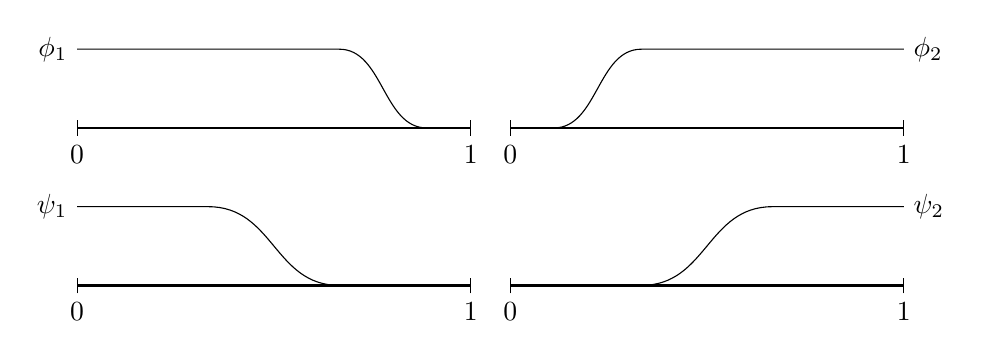
\begin{tikzpicture}[xscale=5]
      \draw [thick] (0, 0) -- (1, 0);
      \draw (0, -0.1) node [below] {$0$} -- (0, 0.1);
      \draw (1, -0.1) node [below] {$1$} -- (1, 0.1);
      \draw (0, 1) node [left] {$\phi_1$} -- (0.666, 1) .. controls (0.777, 1) and (0.777, 0) .. (0.888, 0) -- (1, 0);

      \begin{scope}[shift={(0, -2)}]
        \draw [thick] (0, 0) -- (1, 0);
        \draw (0, -0.1) node [below] {$0$} -- (0, 0.1);
        \draw (1, -0.1) node [below] {$1$} -- (1, 0.1);
        \draw (0, 1) node [left] {$\psi_1$} -- (0.333, 1) .. controls (0.5, 1) and (0.5, 0) .. (0.666, 0) -- (1, 0);
      \end{scope}

      \begin{scope}[shift={(1.1, 0)}]
        \draw [thick] (0, 0) -- (1, 0);
        \draw (0, -0.1) node [below] {$0$} -- (0, 0.1);
        \draw (1, -0.1) node [below] {$1$} -- (1, 0.1);
        \draw (1, 1) node [right] {$\phi_2$} -- (0.333, 1) .. controls (0.222, 1) and (0.222, 0) .. (0.111, 0) -- (0, 0);
      \end{scope}

      \begin{scope}[shift={(1.1, -2)}]
        \draw [thick] (0, 0) -- (1, 0);
        \draw (0, -0.1) node [below] {$0$} -- (0, 0.1);
        \draw (1, -0.1) node [below] {$1$} -- (1, 0.1);
        \draw (1, 1) node [right] {$\psi_2$} -- (0.666, 1) .. controls (0.5, 1) and (0.5, 0) .. (0.333, 0) -- (0, 0);
      \end{scope}
    \end{tikzpicture}
  \end{center}
  Importantly, here $\psi_1 + \psi_2 = 1$, and so is a partition of unity.

  Thinking of these as multiplication operators, we set
  \[
    R = \phi_1 Q_1 \psi_1 + \phi_2 Q_2 \psi_2,
  \]
  and standard gluing techniques shows that this works.
\end{proof}

We now know that if we can find a fundamental solution $H$ for $e^{-t D^*D} - e^{-t DD^*}$, then we can calculate
\[
  \idx D = \int_M H_t(x, x)\;\d x
\]
for any $t$. So our job will be to construct $H$ and understand its asymptotic behaviour as $t \to 0$.

As in the previous lemma,  we can construct (approximate) fundamental solutions $H_1$ and $H_2$ near the boundary and in the interior respectively, and set
\[
  K_t(x, y) = H_{1, t}(x, y) \phi_1(x) \psi_1(y) + H_{2, t} \phi_1(x) \psi_2(y).
\]
We see that this satisfies the properties required to run the proof of Theorem \ref{theorem:iterate-fundamental}. So we know there is a true heat kernel $H$ such that $H_t - K_t \to 0$ exponentially as $t \to 0$. So we have
\[
  \idx D \sim \int_{\partial M \times [0, 1]} H_{1, t}(x, x) \psi_1(x) \;\d x + \int_M H_{2, t}(x, x)\psi_2(x)\;\d x.
\]
In the first integral, as $t \to 0$, the contributions of any positive $u$ is exponentially suppressed. So we can replace the integral with one over $\partial M \times \R_{\geq 0}$ and get rid of $\psi_1$.

In the second integral, we know that
\[
  H_{2, t}(x, x) \sim \sum_{k \geq 0} t^{k - d/2} a_k(x),
\]
where $a_k(x)$ are given by local formulas, which are \emph{the same} as the ones in the without boundary case. Moreover, on the collar neighbourhood, $D^*D$ and $DD^*$ are literally equal, both being $-\frac{\partial^2}{\partial u^2} + A^2$ (near the boundary, they are equal as differential operators but have different domains. Here we do not have boundary conditions). So the upshot is $H_{2, t}(x, x) \sim 0$ on the collar neighbourhood, and so we can drop the $\psi_2(x)$ in the integral.

Rearranging these, we know that
\[
  K(t) \sim \idx D - \sum_{k \geq 0} t^{k - d/2} \int_M a_k(x)\;\d x.
\]
We are now in the situation of the end of the previous section. After rearranging, we are allowed to conclude
\[
  \idx D = \int_M a_{d/2}(x) \;\d x - \frac{h + \eta(0)}{2}.
\]

We now apply this to the case where $D$ is the signature operator $\d + \d^*\colon \Omega_+ \to \Omega_-$. We have already found that
\[
  a_{d/2}(x) = L(p_1, \ldots, p_{d/4}).
\]

Recall that $\ker A$ consists of harmonic forms, so
\[
  h = \dim H^*(\partial M),
\]

Combining these with Theorem \ref{theorem:index-sign-boundary}, we deduce that
\[
  \sign M = \int_M L(p) - \frac{h + \eta(0)}{2} + h^-_\infty.
\]

What we have to do now is to do something slightly sneaky. The reason $h^-_\infty$ shows up is that our boundary condition for $D$ required $f_\lambda(0) = 0$ for $\lambda \geq 0$, while the adjoint boundary condition requires it for $\lambda < 0$, and the $\lambda =  0$ case is not treated ``symmetrically''.

We can run the whole calculation all over again where the boundary condition for $D$ is now $f_\lambda(0) = 0$ for $\lambda > 0$. The main difference is that in the formula for $K(t)$, we now declare $\sign 0 = -1$ instead of $+1$. Then the result is that
\[
  \sign M = \int_M L(p) - \frac{-h + \eta(0)}{2} - h_\infty^+.
\]
Subtracting these two equations give
\[
  h = h_\infty^- + h_\infty^+.
\]
Knowing also that $h_\infty^{\pm} \leq \frac{h}{2}$, we know that they must in fact be equal. So we get
\begin{thm}
  \[
    \sign M = \int_M L(p) - \frac{\eta(0)}{2}.\fakeqed
  \]\ifplastex\fakeqed\fi
\end{thm}

\appendices
\section{Index and Geometry}\label{section:index-and-geometry}
In this appendix, we briefly demonstrate how interesting topological invariants can be expressed as the index of a differential operator.

We recall some basics. Fix a manifold $M$ and bundles $E, F \to M$, together with an elliptic differential operator $D\colon \Gamma(E) \to \Gamma(F)$. Then $\ker D$ and $\coker D$ are finite-dimensional, and the \emph{index} of $D$ to be
\[
  \idx D = \dim \ker D - \dim \coker D.
\]
$D$ has a formal adjoint $D^*$, and $\coker D \cong \ker D^*$. So
\[
  \idx D = \dim \ker D - \dim \ker D^*.
\]

Usually, the operator $D^*D$ is more recognizable. If $\psi \in \ker D^*D$, then
\[
  0 = (\psi, D^*D\psi) = (D\psi, D \psi).
\]
So $\ker D = \ker D^*D$. Then we can write
\[
  \idx D = \dim \ker D^*D - \dim \ker DD^*.
\]

The Hodge decomposition theorem allows us to relate the kernel of differential operators to something more topological.

\begin{thm}[Hodge decomposition theorem]
  Let $M$ be a Riemannian manifold. Recall that the Laplacian on $p$-forms is defined by
  \[
    \Delta = \d\d^* + \d^*\d = (\d + \d^*)^2.
  \]
  If $\psi \in \Omega^p(M)$ is such that $\Delta \psi = 0$, then, as above, $\d \psi = \d^* \psi = 0$. So $\psi$ is in particular a closed form. This defines a map
  \[
    \ker \Delta \to H^*(M).
  \]
  The Hodge decomposition theorem states that this map is an isomorphism.
\end{thm}

Note that $\d + \d^*: \Omega \to \Omega$ is self-adjoint, so its index is just zero. However, by varying its domain and codomain, we can get interesting indices.
\begin{eg}
  Write
  \[
    \Omega_{\mathrm{even}} = \bigoplus \Omega^{2k},\quad \Omega_{\mathrm{odd}} = \bigoplus \Omega^{2k + 1}.
  \]
  Then we have a map
  \[
    \d + \d^*: \Omega_{\mathrm{even}} \to \Omega_{\mathrm{odd}}.
  \]
  The index is then
  \[
    \dim \ker \Delta|_{\Omega_{\mathrm{even}}} - \dim \ker \Delta|_{\Omega_{\mathrm{odd}}} = \chi(M),
  \]
  the Euler characteristic.
\end{eg}

\begin{eg}
  We can play the same game with the signature. Suppose $\dim M = 4k$. Recall that the Hodge star operator is an endomorphism $\Omega^* \to \Omega^*$ that squares to $1$. Write $\Omega_{\pm}$ for the $\pm 1$ eigenspaces. One can show that $\d + \d^*$ anti-commutes with the Hodge star, so induces a map
  \[
    \d + \d^*: \Omega_+ \to \Omega_-.
  \]
  We claim the index of this is exactly the signature of $M$.

  We focus on the kernel of this map; the cokernel is similar. The kernel is the subspace of $H^*(M)$ that is invariant under the Hodge star operator. This consists of the $+1$ eigenspace in $H^{2k}(M)$ plus the subspace spanned by $\psi + *\psi$ for $\psi \in H^{2k - \varepsilon}(M)$ with $0 \leq \varepsilon < 2k$.

  Similarly, the kernel of $\d + \d^*: \Omega_- \to \Omega_+$ consists of the $-1$ eigenspace in $H^{2k}(M)$ plus the subspace spanned by $\psi - *\psi$ for $\psi \in H^{2k - \varepsilon}(M)$ with $0 \leq \varepsilon < 2k$.

  When we subtract the two, we are left with the difference between the $\pm 1$ eigenspaces of $H^{2k}(M)$, i.e.\ the signature.
\end{eg}

\bibliographystyle{alpha}
\bibliography{heat_kernel}

\end{document}
